\chapter{Related Work}
\section{GPU Application Characterization}
Since GPGPU computing exists, there are publications characterizing GPU application. Generally, the analysis
aspects can be separated into high-level and low-level. The former treats an application as a black-box
and measures behaviour of the complete application. The latter inspects hardware level behaviour without
beeing concerned, which part of the application is executed. Most research papers report how changes in software or hardware influence certain aspects of low-level or high-level behaviour.

High-level research often reports speed-up resulting from a change in hardware or software. Abe et al. \cite{6877247} report on power efficiency and performance. 
High-level is also concerned with configuration, such as launch configurations and number of kernels (\cite{6983039}, \cite{Kerr:2009:CAP:1678998.1680778}). Wang et al. \cite{6983039} report on how dynamic programming affects kernel count and launch configurations of irregular workloads. 

Low-level can be devided into memory and execution.
Research concerned with GPU memory behaviour report L2 cache hits/efficiency (\cite{microarch}), global memory load/store counters (\cite{microarch}, \cite{6983039}) or use these numbers together with instruction replay and coalescing to create metrics like memory intensity (\cite{Kerr:2009:CAP:1678998.1680778}) or regularity (\cite{Burtscher:2012:QSI:2473499.2474126}).  Execution research is concerned with control-flow, instruction counts, and occupancy (\cite{microarch}, \cite{Kerr:2009:CAP:1678998.1680778}).

To the best  knowledge of the author, there are no publication researching intra-application interactions of kernels or CTAs.
%\begin{itemize}
%	\item Usually see Application not as a set of different kernels and ignore kernel "interactions"...
%	\item ... or go down to instruction/warp 
%	\item ... or look at architectural impacts on applications
%	\item A Characterization and Analysis of PTX Kernels
%	Andrew Kerr, Gregory Diamos, and Sudhakar Yalamanchili: Broad overview on many applications. Simulated PTX execution, Memory Intesity, branch divergence etc.
%	\item Most other Papers analyse on similar levels, focussing on different Application or Architecture Aspects
%\end{itemize}
\section{GPU Code Instrumentation}
Instrumenting existing application with addition code for memory tracing is essential for this work.
A framework for code instrumentation is presented in "Lynx: A Dynamic Instrumentation System for Data-Parallel Applications on GPGPU Architectures" \cite{Farooqui:2012:LDI:2310660.2310989} by Farooqui et al. Lynx is a framework including a C-to-PTX JIT, that extends CUDA code on PTX level with user defined instrumentation, and a runtime, displayed in \ref{lynx-rt}. The user writes instrumentation specification in a C-style language. The specification is translated to PTX and inserted into the original application.

The application can be instrumented on kernel, basic block and instruction level. An API offers access to CUDA constructs like Thread and CTA IDs, CTA barriers and instruction counts. To increase
efficiency, it is possible that only one thread in a warp performs the specified trace operation. It is possible to access shared and global memory space. The runtime manages all buffers introduced by the instrumentation, including the movement from and to the device.

There are two reasons, Lynx is not suitable for this project. First, while it is possible to instrument global memory operations, we found no way to access details about the instrumented instruction, like target address or type size. However, address information is crucial for this work. The second reason
is the runtime handling the data buffers. As the generated trace data can be very big, device memory would not suffice to hold all the data, and creating a dynamic producer-consumer buffer using Lynx is not possible.
To the knowledge of the author, there is no performance analysis beyond metric counters available for GPUs.
\begin{figure}[t]
	\centering
	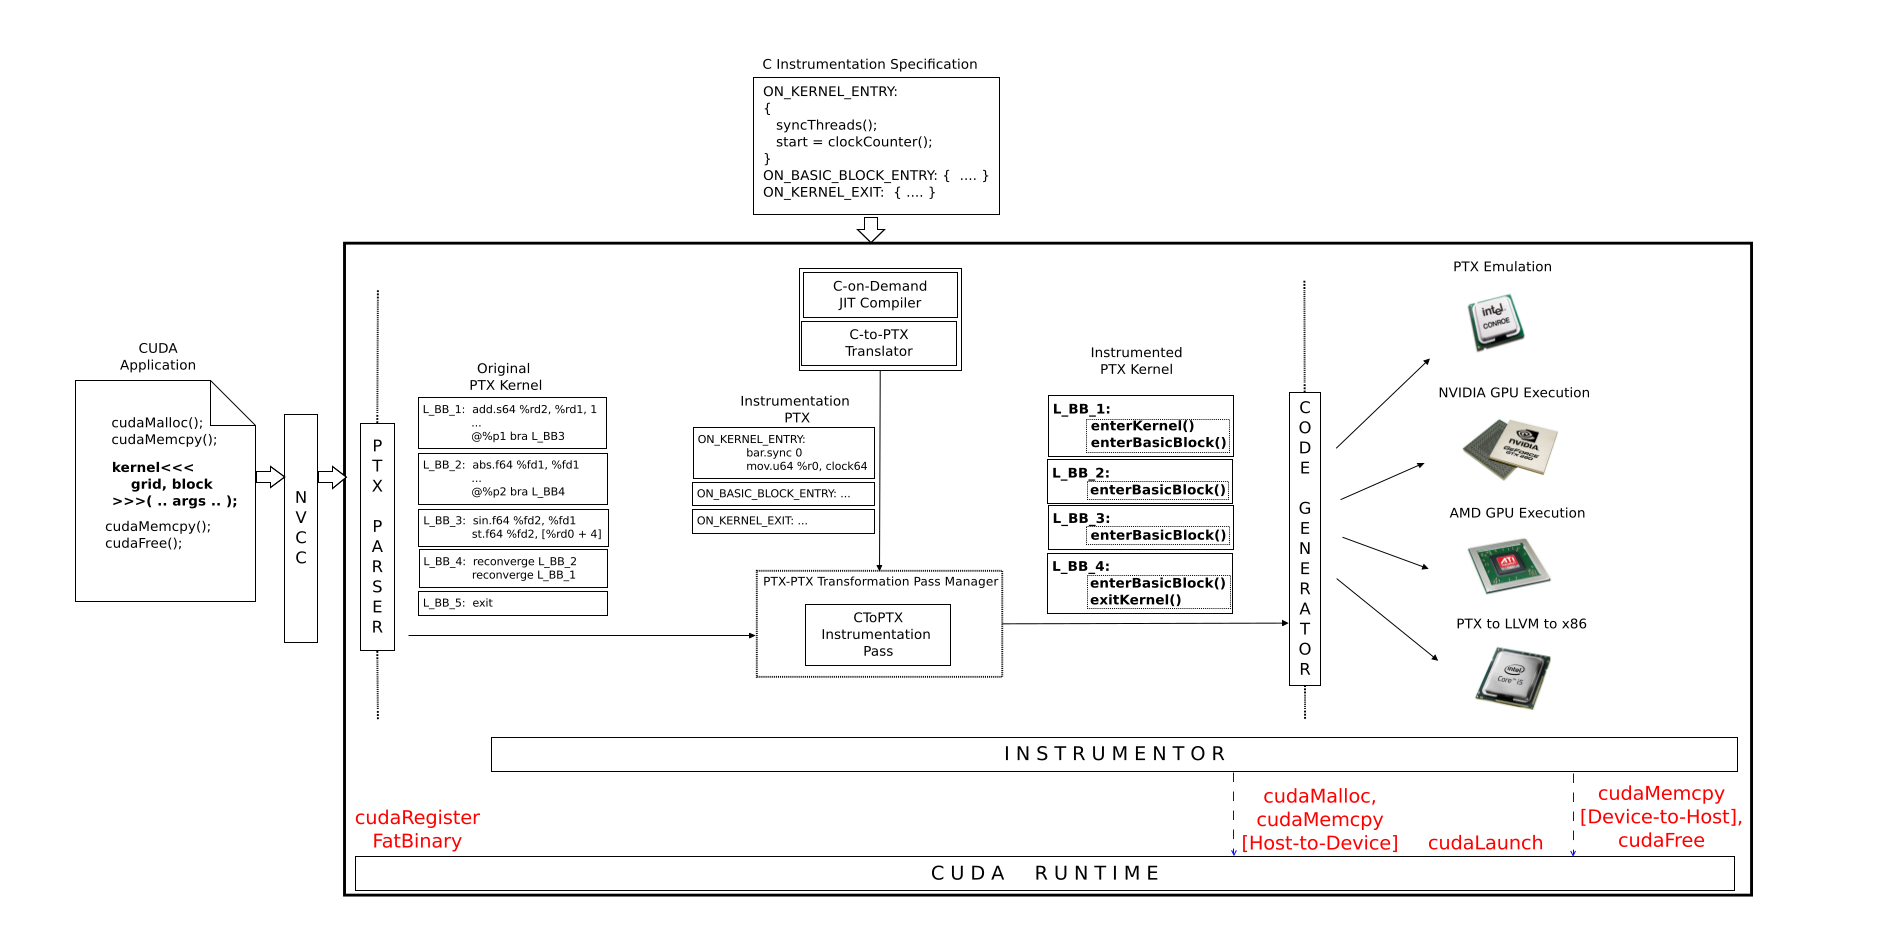
\includegraphics[trim={2.5cm 0 4cm 0},clip,width=\textwidth]{lynx-rt}
	\caption[Lynx Framework]{Lynx framework with all components. The original application is instrumented on PTX level, with code generated by a C-to-PTX JIT from instrumentation specification. Generated data is moved and form the device by the runtime. Image from \cite{Farooqui:2012:LDI:2310660.2310989}}
	\label{lynx-rt}
\end{figure}
%\section{MPI Communication Traces}
%\begin{itemize}
%	\item Not the same because Message Passing != Shared Memory
%	\item Communication Patterns: Rolf Riesen: Paper on Communication Analysis and Patterns, not focussing on special Applications or Architectures. Provides useful metrics to discuss communication
%\end{itemize}